% ************************************************
\chapter{Network Model}\label{ch:Network Model} 
% ************************************************

Referring to anisotropic characteristics in local cortical circuits of
the rat's brain, a network model implementing anisotropic tissue
geometry is developed. The introduction of a rewiring algorithm and
qualitative anisotropy measure %quantitative ??
lay the foundation for the analysis of structural aspects of this
model in Chapter~\ref{ch:structural_aspects}.

%\section{Introduction}\label{sec:intro_model}
\clearpage


% 
% ######################################################################### %
% ------------------------------------------------------------------------- %
%                   Anisotropy in Neural Connectivity
% ------------------------------------------------------------------------- %
% ######################################################################### %


\section{Anisotropy in Neural Connectivity}
\label{sec:biol_anisotropy}

Neurogeometry\index{neuro geometry} addresses the problem of inferring
synaptic connectivity from the geometric shapes of axon and
dendrites. A fundamental concept in this field is that of a
\textit{potential synapse}\index{potential synapse}
\parencite{Stepanyants2002}. Defined as the potential axonal-dendritic
connection of two neurons, present whenever the axon of one neuron is
within a spatial distance $s$ of the dendrite of the other, it is a
necessary, although not sufficient, condition for the formation of a
synaptic connection (\autoref{fig:potential_synapse}). The existence
of such close appositions solely depends on dendritic and axonal
anatomy; identification of defining morphological characteristics in
both axon and dendrite would therefore allow for a model of local
network connectivity, assuming for example that a certain ratio $r$ of
potential synapses turn into active contacts independently. It is the
hope that such a model, motivated from the geometry of a neuron's
functional compartments, not only displays inherent patterns of
connectivity similar to what has been observed in biological networks,
but also proves itself as a testing ground for how this connectivity
may affect network dynamics.

\vspace{-0.21cm}
\definecolor{lightgray}{rgb}{0.88, 0.88, 0.88}
\begin{center}
 \setlength{\fboxrule}{0pt}
 \fcolorbox{black}{lightgray}{
   \begin{minipage}[c]{0.90\textwidth}

     \vspace{0.1cm}
     \setlength{\intextsep}{0pt}%
     \setlength{\columnsep}{8pt}%
     \begin{wrapfigure}{r}{0.65\textwidth}
       \captionsetup{labelformat=empty,labelsep=none}
       \centering
       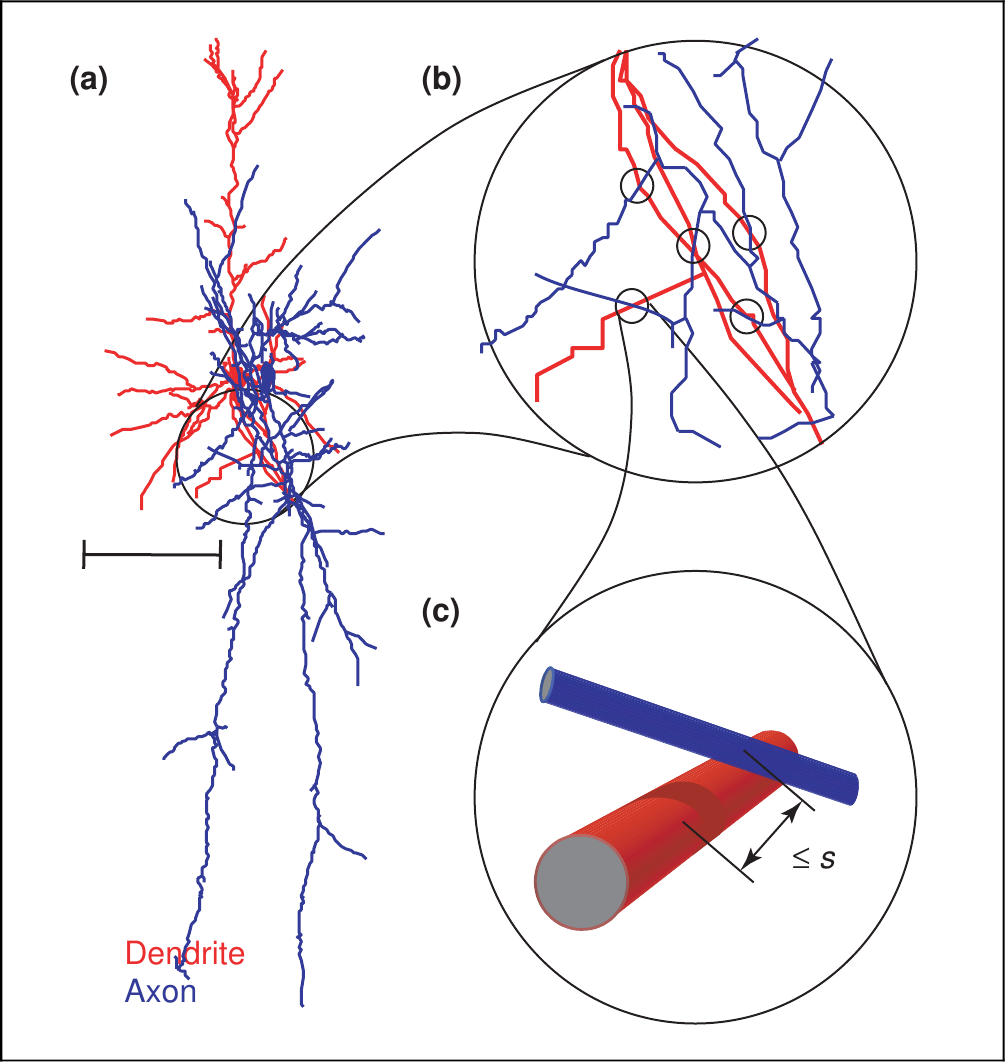
\includegraphics[width=\linewidth]{img/potential_synapse2.png}
       \vspace{-35pt}
       \caption{}
       \label{fig:potential_synapse}
     \end{wrapfigure}

     \footnotesize \textbf{Potential Synapse} 
     \smallskip

     Close ap\-positions be\-tween den\-drite and axon
     are a necessary condition for the formation of a synapse. \textbf{(a)}
     3-D reconstructions of a py\-ra\-mi\-dal cell den\-drite in red, axon of a
     regular spiking non-pyramidal cell in blue. \textbf{(b)-(c)}
     Overlapping arbors allow for several potential synapses whenever
     dendrite and axon are within a spatial distance $\leq s$. Values for
     $s$ depend on the type of synapse, typically between
     0.4-\SI{2}{\micro\meter}. Scale bar: \SI{100}{\micro\meter},
     \SI{30}{\micro\meter}, \SI{3}{\micro\meter} in (a),(b),(c)
     respectively. Image from \textcite{Stepanyants2005}. \hfill \textbf{4.1}

     \vspace{0.1cm}
   \end{minipage}}
\end{center}
%\vspace{-0.12cm}


Finding stereotypical anatomical characteristics however is difficult,
as axonal morphology is, in general, highly diverse
%------------------------------------------------
\marginpar{high variability in axonal morphology} 
%------------------------------------------------ 
\parencite{Debanne2004}. Across different species,
distinct regions in the central nervous system and different neuron
types, axons display a wide variety of shapes characterized by
morphometric parameters such as total length, branching complexity and
axonal extent \parencite{Ropireddy2011}. Typical examples of distinct
morphology include the T-shaped axons of cerebellar granule cells
branching only at a singular point \parencite{Cajal1911}, and axons of hippocampal CA3
pyramidal cells, which, in stark contrast, may feature up to 40
branches resulting in a total length of axon collaterals of up to
\SI{12}{\milli\meter} \parencite{Ishizuka1990}.

It is therefore imperative to confine this analysis to a specific
brain region and neuron type. In this study, we set the focus on
circuits of pyramidal cells in the mammalian cortex.
%?? Cortex does this
%?? Cortex is this well studied
%?? Here we go
More specifically, local circuits of thick tufted layer 5
pyramidal neurons in the rat's somatsosensory cortex have been the
target of advanced
experimentation \parencite{Song2005,Perin2011,Romand2011, Ramaswamy2012}, and will
serve as a benchmark for results in neural morphology and network
connectivity in this report.


\begin{figure}[!htbp]
  \centering 
  \makebox[0.875\textwidth]{%
    \begin{overpic}[width=0.4\textwidth]{%
        img/network_model/p14rr_1.pdf}
      \put(3,92){\small\textbf{A}}
    \end{overpic}
    \hfill
    \begin{overpic}[width=0.4\textwidth]{%
        img/network_model/p14rr_1_axon_traced_soma.pdf}
      \put(3,92){\small\textbf{B}}
    \end{overpic}
    }%
  \caption{\textbf{Tracing axonal branching of a pyramidal cell} In a
    3-D model reconstructed from biocytin-labeled thick-tufted layer 5
    pyramidal cells in the somatosensory cortex of postnatal (day 14)
    Wistar rats, \textcite{Romand2011} depict dendritic compartments in
    red, axonal compartments in blue.  \textbf{A)} A
    \SI{600}{\micro\meter} window centered on the soma of the pyramidal
    cell shows the main stem of the cell's axon projecting downwards in a
    straight line, collaterals branching at various angles. \textbf{B)}
    Using image manipulation software, axon morphology was manually traced
    and is emphasized in black.}    
  \label{fig:romand_axon_trace}
\end{figure}


Axonal morphology of pyramidal cells in the cerebral cortex is well
described. From the soma the single main stem of the axon
%------------------------------------------------
\marginpar{cortical axons form straight lines, arborize profusely} 
%------------------------------------------------ 
originates and projects downwards, describing a trajectory closely
resembling a straight line \parencite{Braitenberg_Cortex}. At
arbitrary points along this path, collaterals branch off at various
angles and constitute themself linear paths until they further ramify
or terminate. Displaying a high degree of ramification, axonal trees
of cortical pyramidal cells build, in general, complex
structures \parencite{Petersen2003,Ramaswamy2012}. Cortical slice
experiments analyzing neural anatomy are typically constrained by a
slice thickness of \SI{300}{\micro\meter}. On this scale, 3-D
reconstruction from labeled thick tufted layer 5 pyramidal cells
reveals characteristic morphology of the axonal tree
(\autoref{fig:romand_axon_trace}). The downwards projecting, straight
axon branches at several points, forming collateral branches that
travel in linear path as well.

In a statistical view, this characteristic axonal morphology results
in high axon branch densities along the main stem, whereas distant
regions display a relatively low density
(\autoref{fig:axon_heat}). Specifically, axon collaterals do not
cluster around the soma but align with the main stem's projection. As
presence of an axonal branch constitutes a necessary condition for a
potential synapse, a higher concentration of potential and,
subsequently, realized synapses is expected in regions of high branch
density. For a coherent picture of local connectivity profiles,
however, dendritic morphology needs to be considered as well. 

 
\begin{figure}[!htbp]
  \centering 
  \makebox[0.875\textwidth]{%
    \begin{overpic}[width=0.4\textwidth]{img/network_model/p14rr_1_trace_soma.pdf}
      \put(3,92){\small\textbf{A}}
    \end{overpic}
    \hfill
    \begin{overpic}[width=0.4\textwidth]{img/network_model/axon_heat_correct_soma.png}
      \put(3,92){\small\textbf{\textcolor{white}{B}}}
    \end{overpic}
    }%
    \caption{%
      \textbf{Illustrating axonal branch density}
      In a sample of 5 reconstructions from thick-tufted layer 5 pyramidal
      cells \parencite{Romand2011}, tracing axonal morphology illustrates
      characteristic branch density along the axon's main
      stem. \textbf{A)} Example of extracted axonal tree. Outline manually
      traced using image manipulation software. Soma indicated by
      triangle. Original data from \textcite{Romand2011}. \textbf{B)}
      Overlaying 5 axonal trees extracted as in A), 
      % ?? show Appendix?  Sumatra label?? colorbar??
      applying a Gaussian filter and displaying high axon densities in
      warm colors, illustrates the characteristic higher branch
      densities along the axon's main stem.}
  \label{fig:axon_heat}
\end{figure}


Dendritic anatomy of cortical pyramidal cells is inherently bipartite.
From the soma several \textit{basal dendrites}\index{basal dendrite}
emerge and extend into arbitrary directions, branching profusely until
they terminate . The single \textit{apical dendrite}\index{apical
  dendrite} emerges from the apex of the pyramidal cell and ascends in
a linear trajectory, forming occasional collateral branches until
finally terminating into the apical tuft, where the dendrite branches
several times to form a tree like structure \parencite{Feldman1984}.
%------------------------------------------------
\marginpar{basal dendrites dominate local connectivity} 
%------------------------------------------------  
On the scale of typical cortical slice thickness, however, the apical
dendrite is cut off and the basal dendrite dominates the dendritic
morphology and potential of dendritic-axonal connections
(\autoref{fig:dendrite_heat}). The radial extension of dendritic
branches results in a high concentration of dendritic branches around the
soma, much in the contrast to the findings of axonal branch densities
before.

\begin{figure}[!ht]
  \centering
  \makebox[0.875\textwidth]{%
    \begin{overpic}[width=0.4\textwidth]{%
        img/network_model/p14rr_1.pdf}
      \put(3,92){\small\textbf{A}}
    \end{overpic}
    \hfill
   \begin{overpic}[width=0.4\textwidth]{img/network_model/p14rr_1_traced_soma.pdf}
      \put(3,92){\small\textbf{B}}
    \end{overpic}
    }
  \vfill
  \vspace{0.3cm}
  \makebox[0.875\textwidth]{%
    \begin{overpic}[width=0.4\textwidth]{img/network_model/p14rr_1_dendrite_trace_scale.pdf}
      \put(3,92){\small\textbf{C}}
    \end{overpic}
    \hfill
    \begin{overpic}[width=0.4\textwidth]{img/network_model/dendrite_heat_correct_soma.png}
      \put(3,92){\small\textbf{\textcolor{white}{D}}}
    \end{overpic}
    }%
  \caption{\textbf{Dendritic morphology and branch density}
    Using neuronal morphology of thick-tufted layer 5
    pyramidal cells recorded by \textcite{Romand2011}, dendritic
    anatomy is traced and combined to illustrate high
    branch density around the soma. \textbf{A)} In a
    \SI{600}{\micro\meter} window centered on the soma, basal
    dendrites (red) are visible extending around the soma. The ascending
    thick apical dendrite (red) is cut off and apical tuft is not
    shown. \textbf{B)-C)} Manual tracing of dendritic outlines
    in five samples (one shown), allows for clearer identification of
    stereotypical morphology and later analysis. \textbf{D)} Combining
    5 dendritic outlines as shown in C) and subsequent Gaussian
    filtering reveals the relatively high dendritic branch density
    around the soma.
  }%?? sumatra label
  \label{fig:dendrite_heat}
\end{figure}


Combining the above results of dendritic and axonal branch densities
in the light of neurogeometry, a clear concept of anisotropy of neural
connectivity emerges. As dendritic branches of potential post-synaptic
targets extend radially from the soma and do not display a preferred
direction, target neurons for outgoing synaptic contacts originating
from a single pyramidal cell, cluster around the downwards projecting
axon (\autoref{fig:neural_anisotropy}). %?? high branch density
                                %correlates directly with expected
                                %number of contacts!
\begin{figure}[!ht]
  \centering 
  \makebox[0.875\textwidth]{%
    \begin{overpic}[width=0.4\textwidth,frame]{img/network_model/axon_dendrite_meet.pdf}
      \put(3,92){\small\textbf{A}}
    \end{overpic}
    \hfill
    \begin{overpic}[width=0.4\textwidth,frame]{img/network_model/axon_dendrite_meet_schema_dense.pdf}
      \put(3,92){\small\textbf{B}}
    \end{overpic}
    }%

    \caption{%
      \textbf{Connected neurons of a single pyramidal cell align with
        axonal projection} Reducing the full axonal (blue,
      cf. \autoref{fig:romand_axon_trace}) and dendritic trees (red, gray,
      cf. \autoref{fig:dendrite_heat}) as shown for two neurons in A)
      to their stereotypical axonal (blue) and dendritic profiles
      (red, gray) in B), demonstrates how connected neurons (red) tend
      to cluster around the pre-synaptic axon's profile, as spatial
      closeness constitutes a necessary condition for the formation of
      contacts. Unconnected neurons (gray) are found distant from the
      axon's projection, but not necessarily distant from the soma. }
  \label{fig:neural_anisotropy}
\end{figure}
%\vspace{-0.2cm} 
% Why is anisotropy so good??
% It becomes apparent that
% connected neurons are located along the main axon in much higher
% concentration than in directions that diverge from the axon's
% projection. 
In their in-depth study, \textcite{Stepanyants2005} confirm the
overrepresentation of potential synapses along the axon for pyramidal
cells. Consistent with the notion that stereotypical morphology of
pyramidal cells is intrinsic to the local network's connectivity
profile, they also find that anisotropy of this degree is \textit{not}
present in spiny stellate neurons located in lower-layer-4.


%%% Local Variables: 
%%% mode: latex
%%% TeX-master: "../dplths_document"
%%% End: 

 % ######################################################################### %
% ------------------------------------------------------------------------- %
%                   Anisotropic geometric network model
% ------------------------------------------------------------------------- %
% ######################################################################### %


\section{Anisotropic Geometric Network Model}
\label{sec:anisotropic_network_model}

Taking up the concept of anisotropy in neural connectivity introduced
in the last section, we propose here, as basis for this study, a
simple geometric network model featuring anisotropic
connectivity. Constructing such a model, we're challenged with
resembling the anisotropic aspects outlined in the last section as
closely as possible, while at the same time basing the model on simple
and abstract relations to allow for an analytical study of such
anisotropic networks.

With this in mind, we propose the following model: On a square surface
of side length $s$, a number of $N$ point neurons are randomly,
uniformly distributed.  Connected neighbors are then calculated for
each neuron separately and independently, by determining the randomly,
uniformly distributed direction of the neuron's single axon. In this
direction the axon traverses over the surface describing a straight
path, terminating only when an edge of the surface is
reached. Directed contacts are made with every neuron that is within a
width $w(x)$ of the axon's trajectory, where in general $w$ depends on
the axon length $x$ at this point
(\autoref{fig:anisotropic_network_model}).

\begin{figure}[!htbp]
  \centering 
  \makebox{%
    \begin{overpic}[width=0.325\textwidth,frame]{%
        img/network_model/model_dendrite_w.pdf}
      \put(3,91){\small\textbf{A}}
    \end{overpic}
    \hfill
    \begin{overpic}[width=0.325\textwidth,frame]{%
        img/network_model/model_axon_w.pdf}
      \put(3,91){%
        \fboxsep=0pt\colorbox{white}{\small\textbf{B}}
        }
    \end{overpic}
    \hfill
    \begin{overpic}[width=0.325\textwidth,frame]{%
        img/network_model/connectivity.pdf}
      \put(3,91){\small\textbf{C}}
    \end{overpic}
    }%
    \caption{%
      \textbf{Anisotropic geometric network model and interpretations
        of width parameter $\boldsymbol w$} Illustrating the process
      of finding connections for one neuron (large triangle, black),
      the axon describes a linear trajectory in an arbitrary direction
      and until terminating on the surface's edge. Target neurons
      (red) are encountered along the path within a (here constant)
      distance $w$, which is in \textbf{A)} interpreted as a dendritic
      radius or, equivalently, in \textbf{B)} as a \enquote{bandwith}
      of the axon. Connections to the encountered targets are then
      established as projections in \textbf{C)}, consistent with the
      directed nature of synapses in biological networks
      (cf. Section~\ref{sec:Biology}).}
  \label{fig:anisotropic_network_model}
\end{figure}

The implementation of arbitrary axonal orientation is crucial to the
model. Although cortical axons are described as consistently
%------------------------------------------------
\marginpar{random axonal orientation yields relevant connectivity} 
%------------------------------------------------ 
projecting downwards \parencite[%
cf. Section~\ref{sec:biol_anisotropy}]{Braitenberg_Cortex}, combining
exclusively vertically aligned axons with the simplified axonal and
dendritic morphological profiles would result in a \enquote{vertically
  staggered connectivity} - neurons could then only project to targets
located below them.  It is in fact not a vertical alignment of axon
orientation, but the anisotropy in neural connectivity - the
observation of neuronal targets aligning with the axonal projection -
that we try to capture and analyze in this model. 

We will refer to the model as the \textit{anisotropic geometric
  network model}. Trying to provide a simple, abstract model isolating
anisotropy in connectivity, in most of this study the width $w(x)$ is
assumed to be constant, $w(x) =w$, a notable exception being the
development of tuned networks in Section~\ref{sec:tuned_networks}. In
the graph theoretic context the anisotropic network model is a random
graph model, in which a realization of the random process results in a
geometric directed graph with a special mode of connectivity. We can
formally define such realization as:

\begin{definition}[Anisotropic geometric graph]
  \label{def:anisotropic_geometric_graph} 
  \index{anisotropic geometric!graph} %
  Let $n \in \mathbb{N}$ and $w \in (0,\infty)$. An
  \textit{anisotropic geometric graph} $G_{n,w}$ then consists of a
  tuple $(G,\Phi,a)$, of a simple directed graph $G$ with $|V(G)|=n$
  vertices and the maps $\Phi:V(G)\to[0,1]^2$ and $a:V(G)\to[0,2\pi)$,
  such that for every vertex pair $v,v' \in V(G)$ and edge $e\in E(G)$
  with $s(e)=v$ and $t(e)=v'$ exists if and only if the inequalities
  for scalar products
  \[
    R_{-a(v)}\left(\Phi(v')-\Phi(v)\right)\hat{e}_x \geq 0 
      \quad \mathrm{and} \quad
    \abs{R_{-a(v)}\left(\Phi(v')-\Phi(v)\right)\hat{e}_y} 
      \leq \frac{w}{2}
  \]
  hold. Here $R_{\varphi}$ is the rotation matrix of angle $\varphi$
  in the Cartesian plane and $\hat{e}_x, \hat{e}_y$ are the standard
  unit vectors. % ?? Alpha or A??
  % for $y=A_{\alpha(v)}(v'-v)$ the identities $y\hat{e}_x > 0$
  % and $\abs{y \hat{e}_y} \le \frac{w}{2}$ hold.
\end{definition}

The anisotropic random graph model then is then giving the probability
distribution over the set of anisotropic random graphs by describing a
random process generating such graph.

\begin{definition}[Anisotropic random graph model]
  \index{anisotropic geometric!random graph model} 
  Let $n \in \mathbb{N}$ and $w > 0$. The \textit{anisotropic random
    graph model} $G(n,w)$ is a probability space over the set of
  anisotropic geometric graphs with a probability distribution induced
  by the following process: Let $G$ be an empty graph with $n$
  vertices. Assign randomly and uniformly to every vertex $v \in V(G)$
  a position $\Phi(v) \in [0,1]^2$ and axonal orientation $0\leq a(v)
  < 2\pi$. Then add edges such that $(G,\Phi,a)$ is an anisotropic
  geometric graph $G_{n,w}$.
\end{definition}


As with every geometric graph model introduced, we restrict the
surface to be the unit square. This does not limit the model, as only
the relative width of the axon band in regard to the surface's side
length is determining connectivity statistics -
%------------------------------------------------
\marginpar{anisotropic model independent of scaling} %
%------------------------------------------------ 
the expected number of connections is easily obtained by the quotient
of the area covered by the axon and the surface area, making
connectivity statistics in the anisotropic random graph model
essentially \enquote{scale-free}.

The following maybe interpreted as a study of anisotropic geometric
graphs in the light of a neuroscientific context. To enable such an
analysis, a few more concepts are needed. The introduction of
those concepts composes the rest of the chapter. A first important
step is the numerical implementation of the anisotropic network model.



%%% Local Variables: 
%%% mode: latex
%%% TeX-master: "../dplths_document"
%%% End: 
% 

% ######################################################################### %
% ------------------------------------------------------------------------- %
%                         Numerical Implementation
% ------------------------------------------------------------------------- %
% ######################################################################### %


\section{Numerical Implementation}\label{numerical_implementation}

Numerical implementation of the anisotropic random graph model was
achieved in Python\footnote{Python Software Foundation. Python
  Language Reference, version 2.7. Available at
  \url{http://www.python.org}}. Relying on NumPy as part of the
scientific Python library SciPy\footnote{Eric Jones, Travis Oliphant,
  Pearu Peterson and others. NumPy version 1.6.1. Available at \url{http://www.scipy.org}}
for the more complex mathematical computations, the implementation
also uses graph-tool\footnote{Tiago
  P. Peixoto. Efficient network analysis. Version 2.2.18. Available at
  \url{http://graph-tool.skewed.de/}}, to ensure convenient and
efficient handling of the created networks.

The algorithm for the generation of anisotropic networks closely
resembles Definition~\ref{def:anisotropic_geometric_graph}. After
randomly distributing $N$ neurons on the square of side-length $s$,
for every neuron a random axon horientation $a \in [0,2\pi)$ is chosen
and an affine transformation, such that the current neuron is located
at the origin and its axon projection aligns with the positive x-axis,
secures a straightforward implementation of connectivity, using the
the inequalities in Definition~\ref{def:anisotropic_geometric_graph}
as a rule for establishing connections.

To harness the numerical implemenation to generate networks, a set of
parameters needs to be chosen. The network size $N$ strongly
influences the needed computational efforts in calculations based on
the generated graphs and has thus been set to $N = 1000$. 
%------------------------------------------------
\marginpar{parameter set chosen to resemble cortical circuits}
% ------------------------------------------------
Choosing the surface side-length arbitrarily as $s=100$, the axon
width $w$ determines connectivity in the network, the relation between
width $w$ and overall connection probability $p$ being shown in
\autoref{fig:determine_axon_width}.  In their analysis of connectivity
of thick-tufted layer V pyramidal cells in neonatal rats (day 14),
\textcite{Song2005} report an overall connection probability of
$p=0.116$, consistent with prior reports of a cortical connection
probability of $p \approx 0.1$. Choosing $w$ to be constant, we
determine the axon width such that overall connectivity matches the
value report by Song et al. and obtain $w/2 = 12.6$
(\autoref{fig:determine_axon_width}).

\begin{figure}[htp]
  \centering
  \makebox{%
    \begin{overpic}[width=0.5\textwidth]{%
        plots/c5b64f3e.pdf}
      \put(22.5,57.5){\small\textbf{A}}
      %\put(12,5){\small\textbf{A}}
    \end{overpic}
    \hfill
    \begin{overpic}[width=0.5\textwidth]{%
        plots/585a946f.pdf}
      \put(24.5,57.5){\small\textbf{B}}
      %\put(12,5){\small\textbf{B}}
    \end{overpic}
  }%
  \vspace{-0.15cm}
  \caption{\textbf{Axon width dependent connection probability
      determines parameter for numerical analysis} Generating
    anisotropic networks with different axon widths $w$ and extracting
    probability $p$ of directed connection between two random nodes,
    demonstrates the dependency of $p$ on the width parameter $w$.
    \textbf{A)} At an axon width of over $w=100$, exceeding the
    square's side length, the connection probability saturates at
    $p=0.5$, as axon bands are essentially \enquote{cutting} the
    square in a connected and unconnected half
    (\smtcite{c5b64f3e}). \textbf{B)} For small $w$ the connection
    probability is a linear function of $w$, allowing the width $\nicefrac{w_S}{2}$
    at which $p(w_S)=11.6$ to be determined by a linear fit as
    $\nicefrac{w_S}{2} =
    12.6$ (\smtcite{585a946f}).} %?? fix width issue!!
  \label{fig:determine_axon_width}
\end{figure}



\label{sample_graphs}Having determined a suitable set of parameters as
$N=1000$, $s=100$ and $w=25.2$, we generate 25 graphs with this parameter
set (label: \smtcite{N1000w\char`_ax126-flat\char`_graph0-24}).
%------------------------------------------------
\marginpar{sample graphs as reference for structural analysis}
%------------------------------------------------ 
This set of sample graphs will serve as a reference for the following
structural analysis. Extending the set by the (partially) rewired
sample graphs (see Section~\ref{sec:rewiring}) we obtain a resourceful
reference for the analysis of structural features of anisotropic
geometric graphs, that we will frequently employ to obtain
quantitative and qualitative results.











% \cite{Thomson2002} Axons are not looking for their targets but
% dendrites might, further evidence to focus on axon geometry.


%%% Local Variables: 
%%% mode: latex
%%% TeX-master: "../dplths_document"
%%% End: 


% \clearpage
% \newpage

% % ######################################################################### %
% ------------------------------------------------------------------------- %
%                    Distance dependent connectivity
% ------------------------------------------------------------------------- %
% ######################################################################### %


\section{Distance dependent connectivity}
\label{sec:distance_connectivity}



In Gilbert's random graph model $G(n,p)$,
%------------------------------------------------ 
\marginpar{random graph
  models in Section~\ref{sec:random_graph_theory}}
%------------------------------------------------
probability of connection $p$ is independently chosen and a fixed
value for all vertex pairs. The anisotropic geometric graph model
introduced in Section~\ref{sec:anisotropic_network_model} is itself a
random graph model - node positions as well as preferred directions of
connection are uniformly at random distributed. In contrast to
Gilbert's model however, neither is the probability of connection
between a given vertex pair independent of the realization of other
edges in the graph, nor is it a fixed value - probabilities strongly
depend on internode distance in the anisotropic geometric graph model
introduced.

Analyzing dependencies in the anisotropic model, specifically by
identifying prevalent patterns of connectivity and relating these
modes of non-randomness to biological findings, is the main focus of
Chapter~\ref{ch:structural_aspects}. However, such structural
correlations may not necessarily be an inherent feature of the
network's anisotropy - distance dependent connectivity alone, as
imposed by the model's specific geometry, may be the cause for
emerging dependencies. It is therefore a crucial initial task to map
the anisotropic model's distance dependent connection
probability. Inferring connection probability as a function of
internode distance and comparing it with computational results, in
this section we explore distance connectivity of the anisotropic
network model, securing a vital component in the analysis of
structural features.

\begin{theorem} \label{theorem:distance_prof} Let $(G,\Phi, a)$
  represent an arbitrary realization of the anisotropic random graph
  model $G(n,w)$. Define $C:[0,\sqrt{2}] \to [0,1]$ as the
  distance-dependent connection probability profile of $(G,\Phi)$,
  that is such that $C(x)$ is the probability that for a vertex pair
  $(v,v') \in V(G)^2\setminus\Delta_{V(G)}$ in distance $x =
  \norm{\Phi(v)-\Phi(v')}$ the vertex $v$ projects to vertex
  $v'$. Then
  \[
    C(x) = \begin{cases}%
             \frac{1}{2} & \mathrm{for} \,\, x\le w/2 \\
             \frac{1}{\pi}
             \operatorname{arcsin}\left(\frac{w}{2x}\right) &
             \mathrm{for} \,\, x >  w/2. %
           \end{cases}
  \]
\end{theorem} 

\begin{proof}
  Let $v,v'$ be a pair of vertices in $V(G)^2 \setminus \Delta_{V(G)}$
  in Euclidean distance $x$ of each other. The vector difference
  $\Phi(v')-\Phi(v)$ may then be written as $x e^{i\theta}$, with $0
  \leq \theta < 2\pi$. We have 
  \[
    R_{-\alpha(v)} xe^{i\theta} = xe^{i(\theta - \alpha(v))}.
  \]
  Only for suitable combination of $\theta$ and $\alpha(v)$ an edge
  from $v$ to $v'$ exists. Assuming $\alpha(v)$ fixed, we calculate
  the probability of connection depending on the random choice of
  $\theta$. We can assume $\alpha(v) = 0$, otherwise the same argument
  holds for $\theta' = \theta - \alpha(v)$.

  From \ref{def:anisotropic_geometric_graph} we obtain the necessary and
  sufficient conditions
  \[
   x \cos \theta \geq 0 \quad \mathrm{and} \quad \abs{x\sin \theta}
  \leq \frac{w}{2}.
  \]
  Choosing uniformly at random $\theta$ in the range of $[0,2\pi)$,
  the first condition is satisfied with a probability of
  $\frac{1}{2}$. Consider for the second condition $\theta \in
  [0,\pi)$. We have 
  \[ 
  \sin \theta \leq \frac{w}{2x},
  \]
  and for $x \leq \frac{w}{2}$ the inequality holds for all $\theta$
  by definition of $\sin \theta$. In the case of $x > \frac{w}{2}$, we
  note that for the first condition to hold $\theta$ must already be in
  $[0,\frac{\pi}{2})$ and can thus write the second condition $\theta$ as
  \[
    \theta \leq \operatorname{arcsin}\frac{w}{2x},
  \]
  yielding $C(x)$ by combining the considerations above and using the
  symmetry of sine for $\theta$ in the third and fourth quadrant.
  % 
\end{proof}

\vspace{0.2cm}%??
\begin{figure}[h] 
  \centering 
  \makebox[0.8\textwidth]{%
    \begin{overpic}[width=0.35\textwidth]{%
        tikz/geomtr_prb_05.pdf}%
      \put(3,92){\small\textbf{A}}
    \end{overpic}
    \hfill
    \begin{overpic}[width=0.35\textwidth]{%
        tikz/geomtr_prb.pdf}% 
      \put(3,92){\small\textbf{B}}
    \end{overpic}  
  }%
  \caption{\textbf{Illustrating the proof of
      Theorem~\ref{theorem:distance_prof}} Distance-dependent
    connectivity profile $C(x)$ in an anisotropic geometric graph
    calculated from geometric dependencies. \textbf{A)} In the case of
    $x\leq \nicefrac{w}{2}$, target $v'$ may be located anywhere on the
    shown semicircle and therefore receives input from $v$ with
    probability $\nicefrac{1}{2}$. \textbf{B)} For $x > \nicefrac{w}{2}$,
    suitable positions for target $v'$ are dependent on $x$. The
    geometric relation $\sin \theta = \nicefrac{w}{2x}$ leads to the
    distance-dependent connectivity profile as described in
    Theorem~\ref{theorem:distance_prof}.}
  \label{fig:geomtr_prb}
\end{figure}


We can verify this result by computationally extracting the distance
dependencies in the sample graphs generated. 

\begin{figure}[!htbp]
  \centering
  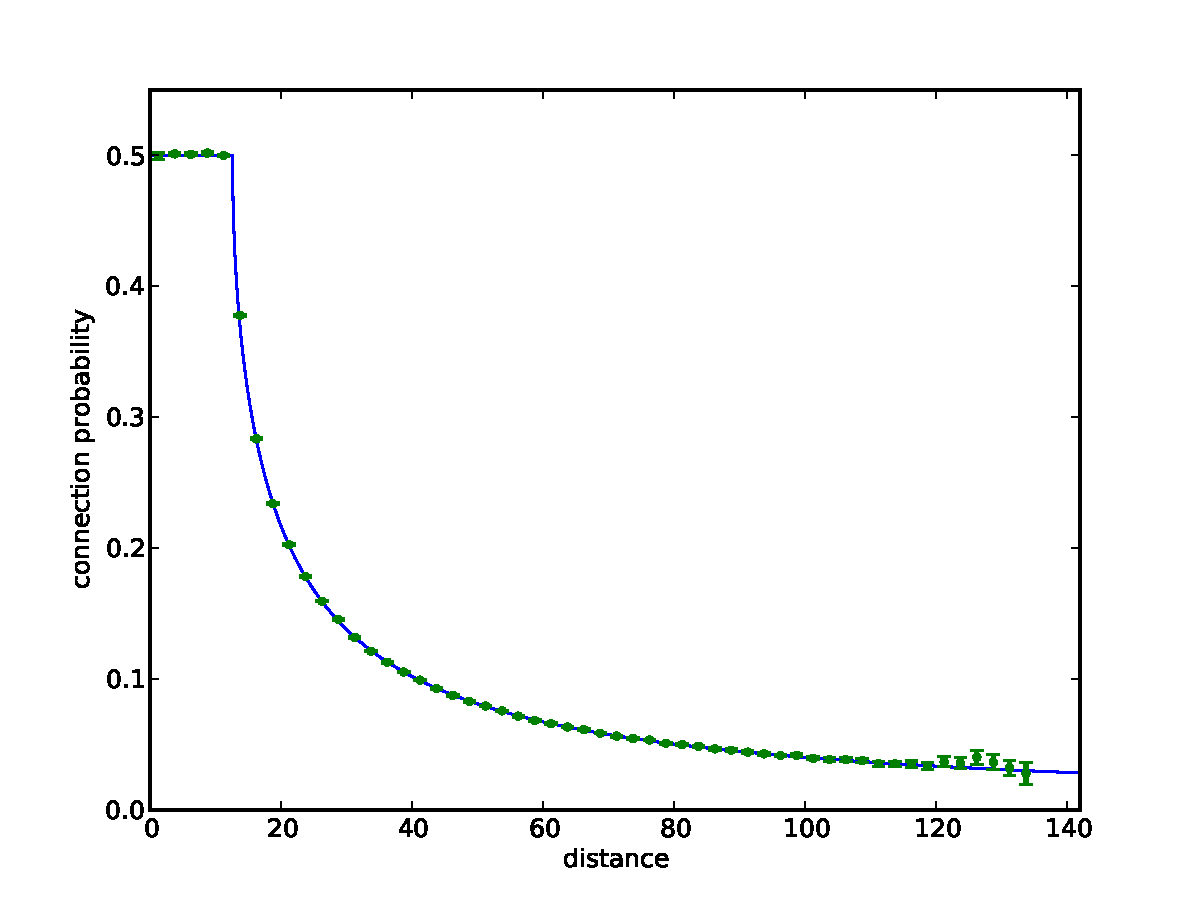
\includegraphics[width=0.8\linewidth]{%
    /users/hoffmann/research/data/sample_graph_analysis/distance_profiles/original/test.pdf} %??
  \caption{\textbf{Predicted distance-dependent connection probability
    profile is matched by numerical computation} In a
    3-D model reconstructed from biocytin-labeled thick-tufted layer V
    pyramidal cells in the somatosensory cortex of postnatal (day 14)
    Wistar rats, \textcite{Romand2011} depict dendritic compartments in
    red, axonal compartments in blue.  \textbf{A)} A
    \SI{600}{\micro\meter} window centered on the soma of the pyramidal
    cell shows the main stem of the cell's axon projecting downwards in a
    straight line, collaterals branching at various angles. \textbf{B)}
    Using image manipulation software, axon morphology was manually traced
    and is emphasized in black.} %??
  \label{fig:distance_theory_compare}%??
\end{figure}


Create additionally a new distance depenedent network sample graphs
and great! 


%%% Local Variables: 
%%% mode: latex
%%% TeX-master: "../dplths_document"
%%% End: 


% 


% ######################################################################### %
% ------------------------------------------------------------------------- %
%                                Rewiring
% ------------------------------------------------------------------------- %
% ######################################################################### %


\section{Rewiring}\label{sec:rewiring}

% In the network configuration introduced in
% section~\ref{sec:network_model} strong directional anisotropy is
% present: Edges originating from one node \enquote{point in the same
%   direction}, that is they connect to other nodes which cluster around
% a. In this section we introduce an algorithm


% It is in our highest interest to compare results to. 
% %------------------------------------------------
% \marginpar{eliminate anisotropy to find structures connected to it} 
% %------------------------------------------------ 
% To this end we introduce an algorithm that preserves
% distance-dependent connectivity as found in
% Proposition~\ref{distance_prof}, but eliminates anisotropy in network
% connectivity by consecutively rewiring existing connections to new
% suitable targets.


Distance-dependency as identified in the last section may already
account for many of the structural features present in anisotropic
networks. A central question of this study is: What structural aspects
in the network are truly features of the anisotropy in connectivity?
Although a quantitative measure for anisotropy will only be introduced
in the next section, already here we are able to qualitatively observe
the strong directionality in connectivity - edges originating from one
node \enquote{point in the same direction}, effectively aligning with
the orientation of the axonal projection of the source node
(cf. \autoref{fig:anisotropic_network_model}). 
%------------------------------------------------
\marginpar{eliminate anisotropy to find structures caused by it} 
%------------------------------------------------ 
To answer the question above, we need to introduce a method that
eliminates this directionality, making networks essentially isotropic
in connectivity. Then, structural features present in the original
anisotropic networks, but not in their rewired, isotropic counterparts
may be attributed to anisotropy.

Rewiring as introduced here, provides the transition from anistropic
connectivity to networks isotropic in connectivity, closely resembling
purely distance-dependent networks. Applying this process only
partially then allows us to analyse structural features as they change with
a varying degree of isotropy, asserting the importance of this process
to our study. In designing the specific rewiring algorithm we identify
two requirements that our implementation should satisfy: 
%\vspace{-3pt}
\begin{enumerate}
  \itemsep-11pt
  \item elimination of anisotropy in connectivity 
  \item preservation of distance-dependent connectivity
\end{enumerate}
%\vspace{-3pt}%
The second point is especially important to us, as we want to impose
isotropy on the network at \enquote{minimal cost}, that is by changing
as little as possible about the other characteristics of the network's
connectivity. The following process respects both of the points above:
\begin{blockquote}{
For every edge between vertices $v$ and $v'$ with inter-vertex
distance $x$, identify neurons with distance to $v$ in the range of
$(x-\varepsilon, x+\varepsilon)$ as potential new targets. Then pick
at random one of these vertices (including $v'$) as a new target for
the current edge, if such an edge doesn't already exist
(\autoref{fig:distance_rewiring}).}
\end{blockquote}
In the graph theoretic context we
formally define a rewiring as follows:

\vspace{0.2cm}
\begin{figure}[H]
  \centering 
  \makebox[0.875\textwidth]{%
    %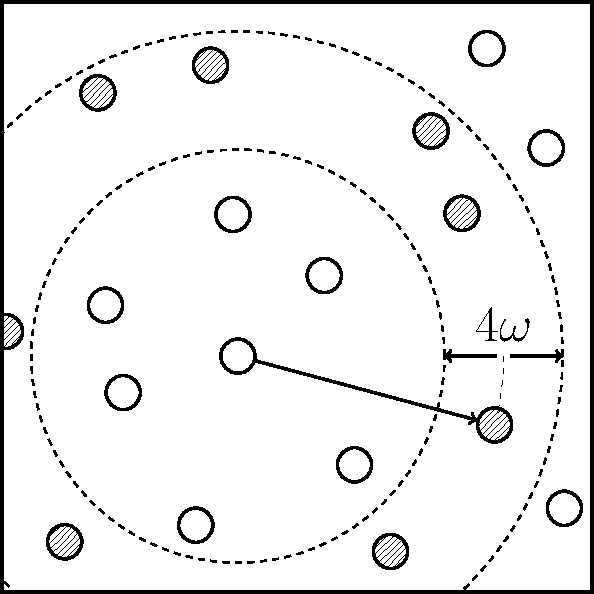
\includegraphics[width=0.4\textwidth]{dist_rew_org.pdf}%
    \begin{overpic}[width=0.4\textwidth, frame]{%
        tikz/distance_rewire_L3.pdf}
      \put(2,102){\small{Before}}
    \end{overpic}
    \hfill
    \begin{overpic}[width=0.4\textwidth, frame]{%
        tikz/distance_rewire_L4.pdf}
      \put(2,102){\small{After}}
    \end{overpic} 
  }%
  \caption{\textbf{Rewiring transforms anisotropic geometric graphs to
      networks with isotropic connectivity} For a given edge $e$ with
    a distance $x$ from its source vertex $v$ to its target vertex
    $t(e)$, potential new targets (striped) are found in within a
    distance $(x-\varepsilon, x+\varepsilon)$ of $v$. The rewired edge
    then projects from $v$ to a new target $t'(e)$, randomly chosen
    from the set of vertices within in this range. Inter-vertex
    distance between $v$ and $t'(e)$ differs by less than
    $\varepsilon$ from $x$, ensuring that for small $\varepsilon$ the
    original distance-dependent connectivity is preserved. (Note that
    all targets within range are eligible for rewiring as no other
    edges exist. In general this is not the case.)}
  \label{fig:distance_rewiring}
\end{figure}


\begin{definition}
  \label{def:rewiring}
  Let $G$ be an anisotropic geometric graph with $\abs{V(G)} =
  n$. Then we define a \textit{rewiring} of $G$ to be probability space over
  $G^n_{\Phi}$, induced by the following process: For every edge $e
  \in E(G)$ uniformly at random pick a potential new target $t'(e)$
  from the set $M_e = T_e \setminus K_e$, where $T_e$ is the set of all
  vertices that differ in their distance to $s(e)$ less than
  $\varepsilon$ from the distance of $s(e)$ to $t(e)$,
  \[ 
  T_e = \left\{v \in V(G) \setminus s(e) \mid \abs{\mathrm{d}(s(e),v)
      - \mathrm{d}(s(e),t(e))} < \varepsilon \right\} %?? definition
                                %of distance d?
  \]
  and $K_e$ the set vertices that already are connected to $s(e)$ by
  another rewired edge, 
  \[
  K_e = \left\{v \in V(G) \mid \exists\, e' \in E'(G): s(e') = s(e),
      t(e') =v \right\},
  \]
  where $E'(G)$ is the set of all edges that have been rewired already.
\end{definition}

Note that in the way Definition~\ref{def:rewiring} is formulated, it
is possible for $M_e$ to be empty for some edge $e$. In this case no
new edge is realized and the resulting, rewired network has
$\abs{E(G)}-1$ edges. In practice this happens negligibly seldom, out
of approximately on average only $25.68$ edges, with a standard deviation
of $4.51$ and accounting for roughly $0.02\%$ of the rewired edges, are \enquote{lost}
in this process (\smtcite{4afc2727}). 

We formulated Definition~\ref{def:rewiring} in such a way, that
distance-dependent connectivity is preserved. We verify this claim by the
following estimation:

Let $\tilde{C}(x)$ be the distance-dependent connectivity profile of a
rewiring $R_{\varepsilon}$ of an anisotropic graph $G_{n,w}$. Denote
with $C(x)$ the distance-dependent connection probability of the
$G_{n,w}$. The expected value for $\tilde{C}(x)$ at any point $x$ We
estimate the expected difference between $\tilde{C}(x)$ and $C(x)$ at
any point $x$ as
\begin{align}
  \mathbf{E}\left[\tilde{C}(x) - C(X)\right]  
    & = \int_{x-\varepsilon}^{x+\varepsilon} f(x') C(x') \, dx -
        C(x)\notag\\
    & = \frac{1}{2\varepsilon}\int_{x-\varepsilon}^{x+\varepsilon}
        C(x') - C(x) \, dx \notag\\
    & = \frac{1}{2\varepsilon} \left\{ \int_{x-\varepsilon}^{x} C(x') -
        C(x) \, dx - \int_x^{x+\varepsilon} C(x') - C(x) \, dx
        \right\} \notag\\
    & = \frac{1}{2\varepsilon} \label{eq:rewiring_est}
\end{align}

The rewiring margin $\varepsilon$ thus simultaneously governs how many
new targets are available for each edge and how well
distance-dependency is preserved. Setting $\varepsilon = 1.25$ %??
                                %right value check!
and applying the rewiring algorithm to the 25 sample graphs, we find
that distance-dependent connectivity of the original graphs is matched
(\autoref{fig:rewiring_dst_prf_compare}) while at the same time
ensuring that for any edge $e$ sufficiently many new rewiring targets
are available (\autoref{suppfig:rew_stats}).

\begin{figure}[H]
  \centering
  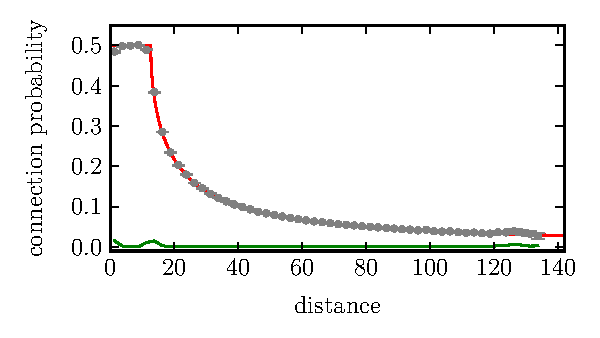
\includegraphics[width=0.8\linewidth]{%
    plots/4f4dfcf1.pdf} 
  \captionsetup{skip=0pt}
  \caption{\textbf{Rewiring with \boldmath$\varepsilon = 1.25$
      preserves distance-dependent profile in sample graphs} Comparing
    the distance-dependent connection probabilities of the original
    graph (Theorem~\ref{theorem:distance_prof}) in red with extracted
    of probabilities from the rewired ($\varepsilon = 1.25$) sample
    graphs in gray (errorbars SEM) we verify that distance-dependent
    connectivity is preserved when rewiring. The green curve shows the
    expected difference between the original and rewired
    distance profiles as estimated in
    Equation~\ref{eq:rewiring_est}. (\smtcite{4f4dfcf1})}
  \label{fig:rewiring_dst_prf_compare}
\end{figure}


As a generalization of Definition~\ref{def:rewiring}, we define a
partial rewiring $R_{\varepsilon, \eta}$, finding new targets only for
a fraction $\eta$ of all edges:

\begin{definition}Let $\varepsilon > 0$ and $0 \leq \eta \leq 1$. A
  \textit{partial rewiring} $R_{\varepsilon,\eta}$ of an anisotropic
  geometric graph $G_{n,w}$ is then a rewiring $R_{\varepsilon}$ of
  $G_{n,w}$, in which every edge is rewired with a probability of
  $\eta$, otherwise it remains. To avoid the occurrence of multiple
  edges, $K_e$ is then extended to include the targets of all edges
  originating from $s(e)$ that will not be rewired.
\end{definition}

Clearly the result above of  partial rewirings preserve
distance-dependent connectivity. Using the we extend our set of sample
graphs once more adding rewired graphs with rewiring margin
$\varepsilon = 1.25$ %still check??
with fractions $\eta = 0.25$, $\eta = 0.5$, $\eta = 0.75$ and $\eta =
1$, presenting a complete rewiring.




 

% \begin{algorithm}
% Let $N(n,e,w) = (G,P,a)$ be  Then 
% \normalfont
% \begin{algorithmic}%[1] <-- gives line numbers
% \For {$v \in V(N_G)$}
%   \For {$e \in E_{\textrm{out}}(v)$}
%      \State $x \gets \norm{N_P(v)-t(e)}$
%      \State $T \gets \{w \in V(N_G) \mid  x-\varepsilon \leq
%      \norm{N_P(v)-N_P(w)} < x+\varepsilon\}$
%      \State $t(e) \gets \textrm{choice} T$
%   \EndFor
% \EndFor
% \end{algorithmic}
% is defined.
% \end{algorithm}


%%% Local Variables: 
%%% mode: latex
%%% TeX-master: "../dplths_document"
%%% End: 


% \cleardoublepage
% \newpage

% 


% ######################################################################### %
% ------------------------------------------------------------------------- %
%                           Anisotropy Measure
% ------------------------------------------------------------------------- %
% ######################################################################### %


\section{Anisotropy Measure}\label{sec:anisotropy_measure}

In the last section a method to rewire an anisotropic geometric graph,
such that was introduced. From an . In this chapter we
introduce.. capturing ..

The $G_{n, \Phi}$ be a geometric graph. Then, for every is the
\textit{preferred direction} and its length is \index{preferred direction}

\textcite{Mardia_Directional-statistics}
 
\begin{figure}[H]
\caption{\textbf{illustrate varying levels of anisotropy}}
\end{figure}


\begin{figure}[H]
  \centering
  \makebox[0.75\textwidth]{%
    \renewcommand{\tabcolsep}{2pt}
    \setlength\extrarowheight{0pt}
    \begin{tabular}{ccc}
      \begin{overpic}[width=0.28\textwidth]{%
          plots/038f5b8c.pdf}
         \put(10,57){\small $\eta = 0$}
      \end{overpic}
      &
      \begin{overpic}[width=0.28\textwidth]{%
          plots/9893ab1f.pdf}
        \put(10,57){\small $\eta = 0.25$}
      \end{overpic}
      &
      \begin{overpic}[width=0.28\textwidth]{%
          plots/0c429f3c.pdf}
        \put(10,57){\small $\eta = 0.5$}
      \end{overpic}
      \\
      \begin{overpic}[width=0.28\textwidth]{%
          plots/400a41bc.pdf}
        \put(10,57){\small $\eta = 0.75$}
        \put(4,-4){$0$}\put(90,-4){$1$}
      \end{overpic}
      &
      \begin{overpic}[width=0.28\textwidth]{%
          plots/a5f54cb4.pdf}
        \put(10,57){\small $\eta = 1$}
        \put(4,-4){$0$}\put(90,-4){$1$}
      \end{overpic}
      & 
      \begin{overpic}[width=0.28\textwidth]{%
          plots/a5b674f0.pdf}
        \put(11,57){\small distance-}
        \put(11,45){\small dependent}
        \put(4,-4){$0$}\put(90,-4){$1$}
      \end{overpic} 
    \end{tabular}
  }
  %
  \caption{\textbf{Rewiring significantly reduces anisotropy} In data
    taken from the 25 sample graphs (??), vertex isotropy degree
    distribution is shown for the original set of graphs ($\eta = 0$)
    The characteristic highly anisotropic profile found in the
    original is already significantly reduced by partial rewiring;
    anisotropy degree distribution in the fully rewired graphs
    resemble degree distribution of equivalent purely
    distance-dependent networks.}%?? sumatra label
  \label{fig:anisotropy} %??
\end{figure}


... suggesting that fully rewired anisotropic networks do not . There
is however one difference in out-degree as an artifact of boundary
confinment (Section~\ref{sec:degree_distribution}).



%%% Local Variables: 
%%% mode: latex
%%% TeX-master: "../dplths_document"
%%% End: 












% ######################################################################### %
% ------------------------------------------------------------------------- %
%                         Summary and Discussion
% ------------------------------------------------------------------------- %
% ######################################################################### %

\section{Summary and Discussion}













%%% Local Variables: 
%%% mode: latex
%%% TeX-master: "../dplths_document"
%%% End: 
